\chapter{Design and Implementation}
\label{chap:impl}

% preliminary structure:

% 1. architecture
% 2. technical details (memory included)
% 3. modules details


% overview of architecture (.exm -> lexer -> parser -> compiler (code gen) -> .yul code -> solidity compiler -> EVM bytecode)
%                                                            |
%                                                            -> ABI generator

% detailed overview of modules (for example: calldata parsing, compiler (two passes), return data transformer, storage)


% technical details:
%   - memory organization
%     - how variables are stored, dynamic typing
%     - immutability of variables
%     - offset
%   - show events/module args syntax
%   - key features
%     - events
%     - constructor
%     - storage
%     - ABI for public functions
%     - reverts with utf-8 error string
%   - standard functions declaration on demand (transitivity included) and mechanism itself (module responsible for )

This chapter outlines the principal elements of the design of Elixireum compiler. It overviews the technology stack employed in the development process and underscores the pivotal decisions that shaped the architecture of the compiler.


\section{Stack overview}
\label{sec:architecture}
This section rationalize the technology stack used in the project: Elixir, Yul, Solidity compiler.
% TODO: add clarification that Elixir is base of the syntax and source language of the compiler
\subsection{Choice of Elixir}
Here is the rationalization behind the choice of Elixir:
\begin{itemize}
    \item One of the most popular open source blockchain explorers, Blockscout\footnote{\href{https://www.blockscout.com/}{https://www.blockscout.com} -- Official Blockscout website}, is written in Elixir. From this we can say that Elixir is well heard of in Web3 community.
    \item Our team possesses substantial expertise in this programming language.
    \item Elixir is open source so we can easily reuse its machinery for tokenization and parsing Elixireum.
\end{itemize}

\subsection{Choice of Yul}
\begin{itemize}
    \item Initially, our strategy was to compile Elixireum directly into Ethereum Virtual Machine (EVM) bytecode. Subsequently, we pivoted towards an intermediate representation (IR), selecting Yul as IR aligned with our requirements. Advantages from this decision are as follows:
        \begin{itemize}
            \item Compatibility with all EVM versions, eliminating the need for version-specific concerns. 
            \item Avoidance of reimplementing primitives such as function calls, variable and stack management, thereby freeing up resources to enhance the feature set of the language.
            \item Reduced gas consumption facilitated by the optimizer of Solidity compiler.
        \end{itemize}
      Despite these considerations, the choice comes with limitations, notably:
        \begin{itemize}
            \item Dependency on the Solidity compiler for Elixireum.
            \item The unresolved bug\footnote{\href{https://github.com/ethereum/solidity/issues?q=is:issue+is:open+StackTooDeepError}{https://github.com/ethereum/solidity/issues?q=is:issue+is:open+StackTooDeepError}} in the Solidity compiler that appears for large smart contracts written in Elixireum when compiled with the optimizer disabled. The bug results in an inability to operate with a large number of variables or deep stack depths.
        \end{itemize}
      No significant downsides compared to direct compilation to EVM bytecode, since bytecode can be used in Yul directly.

    \item We also considered mapping BEAM (Erlang VM) bytecode to EVM bytecode. However, this option presented significant challenges due to the fundamental architectural and philosophical differences between the two virtual machines. BEAM is specifically tailored for environments that demand high concurrency, distribution, and fault tolerance, and it includes a set of opcodes optimized for these conditions. In contrast, the EVM is designed to run smart contracts within blockchain ecosystems, prioritizing deterministic execution and gas metering to protect against spam and enhance network security. BEAM incorporates specialized instructions for concurrency and distributed processing that do not directly translate to the EVM, because of these distinct focuses.
\end{itemize}

\section{Technical details}

\subsection{Memory organization}
\label{sec:memory_organization}

In our language implementation, we decided to store all runtime variables in the volatile memory of the Ethereum Virtual Machine. This decision is justified by the low gas cost associated with memory operations and the simplicity of implementation. We considered two alternatives: transient storage, which is more expensive than memory, and the stack, which involves more complex management.

In the generated Yul code, a variable is defined as a pointer to the memory location where its value is stored. At this pointer, the first byte is reserved for the type number, and the subsequent bytes contain the value itself for simple cases. For more complex cases, such as lists and tuples, the first byte still indicates the type, followed by a word\footnote{in this context word is 32 bytes} that specifies the count of elements, and then the elements themselves, each stored as an inline variable (type + value). For strings or byte arrays, the first byte indicates the type (1 for strings, 102 for byte arrays), the next word specifies the byte count, followed by the actual bytes.

Since we developed a functional language, one of its fundamental principles is immutability. This means that each assignment operation creates a new variable. In practice, we "forget" the previous pointer, assign a new pointer, and place the variable in a new location. Each new variable should be stored sequentially after the previous one. To achieve this, we define the offset\$ variable in the generated Yul code. This variable holds the memory address where the next variable will be stored. As a workaround for corner cases, we update this variable using the msize() call, assigning the current memory size rounded to one word to the offset\$ variable.

In Elixireum syntax, there are no type specifiers for variables. To handle dynamic types, we established several principles upon which our type system is built:
\begin{itemize}
  \item Return values of public functions must strictly match the specified types; otherwise, a revert\footnote{opcode which stops the current execution and throw an error. All the state changes are reverted} operation will be triggered.
  \item For literals, the type is defined at compile time.
  \item The type is stored in the first byte of the variable.
  \item We defined a standard cast function that developers can use in Elixireum code.

  The following code snippet demonstrates the usage of the cast function:
  \begin{lstlisting}[caption={Example of cast function usage}, language=elixir, label={lst:contract_structure}]
    @spec decimals() :: Types.UInt8.t()
    def decimals() do
      Utils.cast(18, Types.UInt8)
    end  
  \end{lstlisting}
\end{itemize}

The following Elixireum code illustrates a simple case:

\begin{lstlisting}[caption={Elixireum code for simple case}, language=elixir]
  a = 1
  b = 2
\end{lstlisting}

This Elixireum code is translated into Yul code as follows:

\begin{lstlisting}[caption={Generated yul code for simple case}, language=yul]
  let offset$ := msize()      // define offset$, set it to current memory size 
  let a$ := offset$           // define variable as the memory pointer
  mstore8(offset$, 67)        // 67 is int256 type, store it as one byte
  offset$ := add(offset$, 1)  // increase current offset by 1 byte, which is used by type on the line above
  mstore(offset$, 1)          // store the value itself
  offset$ := add(offset$, 32) // int256 value takes 32 bytes

  let b$ := offset$           // define variable as the memory pointer
  mstore8(offset$, 67)        // 67 is uin256 type
  offset$ := add(offset$, 1)  // increase current offset by 1 byte, which is used by type on the line above
  mstore(offset$, 2)          // store the value itself
  offset$ := add(offset$, 32) // int256 value takes 32 bytes
\end{lstlisting}

In this Yul code, offset\$ is initialized to the current memory size. Each variable (a\$ and b\$) is defined as a memory pointer. The type of each variable is stored using mstore8, and the actual value is stored using mstore. The offset is incremented appropriately to account for the type byte and the 32-byte value for each variable.

The following table shows a snippet of the EVM memory for this simple case:

\begin{table}[h!]
  \centering
  \renewcommand{\arraystretch}{1.2} % Reduces the height of the table
  \begin{tabular}{|>{\centering\arraybackslash}m{2cm}|>{\centering\arraybackslash}m{1cm}|>{\centering\arraybackslash}m{1cm}|>{\centering\arraybackslash}m{1cm}|>{\centering\arraybackslash}m{0.75cm}|>{\centering\arraybackslash}m{1cm}|>{\centering\arraybackslash}m{1cm}|>{\centering\arraybackslash}m{1cm}|>{\centering\arraybackslash}m{1cm}|>{\centering\arraybackslash}m{0.75cm}|>{\centering\arraybackslash}m{1cm}|}
  \hline
  \textbf{Addresses} & 0x00 & 0x01 & 0x02 & ... & 0x21 & 0x22 & 0x23 & 0x24 & ... & 0x42 \\ \hline
  \textbf{Values}    & 0x43 & 0x00 & 0x00 & ... & 0x01 & 0x43 & 0x00 & 0x00 & ... & 0x01 \\ \hline
  \end{tabular}
  \caption{EVM Memory snippet for simple case}
  \label{tab:evm_memory}
  \end{table}

An example of handling strings in Elixireum is as follows:

\begin{lstlisting}[caption={Elixireum code for string case}, language=elixir]
  a = "abc" # hex representation of this utf-8 string is 0x616263
\end{lstlisting}
  
The corresponding Yul code generated for this string case is:

\begin{lstlisting}[caption={Generated yul code for string case}, language=yul]
  let offset$ := msize()      // define offset$, set it to current memory size 
  let a$ := offset$           // define variable as the memory pointer
  mstore8(offset$, 1)         // store the type, 1 is the string type
  offset$ := add(offset$, 1)  // increase current offset by 1 byte, which is used by type on the line above
  mstore(offset$, 3)          // store the byte size of the string
  offset$ := add(offset$, 32) // increase current memory pointer by 32 bytes, since the size of the string is 256 bit lenght
  mstore(offset$, 0x6162630000000000000000000000000000000000000000000000000000000000) \\ store the string itself
  offset$ := add(offset$, 3)  // string has length only 3 bytes
\end{lstlisting}

In this Yul code, the variable a\$ is defined as a memory pointer. The type of the variable is stored using mstore8, followed by storing the byte size of the string using mstore. The offset is incremented by the size of the string (3 bytes) after storing the string itself.

The following table illustrates a snippet of the EVM memory for this string case:

\begin{table}[h!]
  \centering
  \renewcommand{\arraystretch}{1.2} % Reduces the height of the table
  \begin{tabular}{|>{\centering\arraybackslash}m{2cm}|>{\centering\arraybackslash}m{1cm}|>{\centering\arraybackslash}m{1cm}|>{\centering\arraybackslash}m{1cm}|>{\centering\arraybackslash}m{0.75cm}|>{\centering\arraybackslash}m{1cm}|>{\centering\arraybackslash}m{1cm}|>{\centering\arraybackslash}m{1cm}|>{\centering\arraybackslash}m{1cm}|}
  \hline
  \textbf{Addresses} & 0x00 & 0x01 & 0x02 & ... & 0x20 & 0x21 & 0x22 & 0x23 \\ \hline
  \textbf{Values}    & 0x01 & 0x00 & 0x00 & ... & 0x03 & 0x61 & 0x62 & 0x63 \\ \hline
  \end{tabular}
  \caption{EVM Memory snippet for string case}
  \label{tab:evm_memory}
  \end{table}

An example of handling lists in Elixireum is as follows:

\begin{lstlisting}[caption={Elixireum code for list case}, language=elixir]
  a = [1, true, "abc"]
\end{lstlisting}
  
\begin{lstlisting}[caption={Generated yul code for string case}, language=yul]
  let offset$ := msize()
  
  // define int256 literal
  let var0$ := offset$
  ...  
  // define bool literal
  let bool_var1$ := offset$
  ...
  // define string literal
  let str2$ := offset$
  ...
  
  // define the list itself
  let a$ := offset$ // define variable as the memory pointer
  mstore8(offset$, 103) // store the list type
  offset$ := add(offset$, 1)
  mstore(offset$, 3) // store the length of the list 
  offset$ := add(offset$, 32) // increase current memory pointer by 32 bytes, since the size of the list is 256 bit lenght
  let ignored_
  ignored_, offset$ := copy_from_pointer_to$(var0$, offset$) // copy int256 variable to the start of the list & update offset$
  ignored_, offset$ := copy_from_pointer_to$(bool_var1$, offset$) // copy bool variable to the list & update offset$
  ignored_, offset$ := copy_from_pointer_to$(str2$, offset$) // copy string variable to the list & update offset$
\end{lstlisting}

In this Yul code the variables var0\$, bool\_var1\$, and str2\$ are defined for the integer, boolean, and string literals, respectively. Then list a\$ is defined. The length of the list is stored using mstore, and the actual values of the list elements are copied into memory using the copy\_from\_pointer\_to\$ function, which updates the offset accordingly.

The following table illustrates a snippet of the EVM memory for this list case:
\begin{table}[h!]
  \centering
  \renewcommand{\arraystretch}{1.2} % Reduces the height of the table
  \begin{tabular}{|>{\centering\arraybackslash}m{3cm}|>{\centering\arraybackslash}m{1cm}|>{\centering\arraybackslash}m{1cm}|>{\centering\arraybackslash}m{1cm}|>{\centering\arraybackslash}m{1cm}|>{\centering\arraybackslash}m{1cm}|>{\centering\arraybackslash}m{1cm}|>{\centering\arraybackslash}m{1cm}|>{\centering\arraybackslash}m{1cm}|>{\centering\arraybackslash}m{1cm}|>{\centering\arraybackslash}m{1cm}|}
  \hline
  \textbf{Addresses} & ... & 0x47 & 0x48 & ... & 0x67 & 0x68 & 0x69 & ... & 0x88 & 0x89 \\ \hline
  \textbf{Values}    & ... & 0x67 & 0x00 & ... & 0x03 & 0x43 & 0x00 & ... & 0x01 & 0x02 \\ \hline \hline
  \textbf{Addresses} & 0x8a & 0x8b & 0x8c & ... & 0xab & 0xac & 0xad & 0xae & ... & ... \\ \hline
  \textbf{Values}    & 0x01 & 0x01 & 0x00 & ... & 0x03 & 0x61 & 0x62 & 0x63 & ... & ... \\ \hline
  \end{tabular}
  \caption{EVM Memory snippet for list case}
  \label{tab:evm_memory_aux} 
  \end{table}

\subsection{Key features}
\label{sec:key_features}

\begin{enumerate}
  \item \textbf{Events\footnote{\url{https://docs.soliditylang.org/en/v0.8.25/abi-spec.html\#events}}}

  Events are essential for highlighting storage changes or other significant events in the lifecycle of a smart contract. They can be easily retrieved from the blockchain after being emitted. Events can be defined and emitted in Elixireum as follows:

  \begin{lstlisting}[caption={Events}, language=elixir, label={lst:calldata_decoding_recursive}]
  @test name: "Test", indexed_arguments: [addr: Types.Address.t()], data_arguments: [value: Types.UInt256.t()]
    ...
  addr = ~ADDRESS(0x0000000000000000000000000000000000000000)
  value = 100
  Event.emit(@test, [addr: addr value: value])
  \end{lstlisting}
  
  \item \textbf{Storage}
  
  Each address in Ethereum has its own associated persistent storage, which functions as a key-value store with 32-byte keys and values. This storage is crucial for maintaining a global state. In Elixireum, storage variables can be specified as a module argument using the @ symbol. The type of the storage variable can be any available type, a mapping, or an inner mapping of any depth.

  \begin{lstlisting}[caption={Storage}, language=elixir, label={lst:calldata_decoding_recursive}]
    @balances type: %{Types.Address.t() => Types.UInt256.t()}
    @totalSupply type: Types.UInt256.t()
    ...
    Storage.store(@totalSupply, 1_000_000) # store the value to the storage
    supple = Storage.get(@totalSupply)     # get the value from the storage
    
    addr_1 = ... # define some address
    Storage.store(@balances[addr_1], 1_000)  # update the @balances mapping for addr_1
    balance = Storage.get(@balances[addr_1]) # get value for addr_1 from @balances
  \end{lstlisting}
  
  \item \textbf{Constructor}

  The constructor is called once, during the deployment of the smart contract. It is used to initialize the contract, set the owner, or define any other storage variables. Essentially, it executes any necessary operations upon contract creation.
  
  \begin{lstlisting}[caption={Constructor}, language=elixir, label={lst:calldata_decoding_recursive}]
    @spec constructor(Types.String.t(), Types.String.t()) :: nil
    def constructor(name, symbol) do
      Storage.store(@name, name)
      Storage.store(@symbol, symbol)
      Storage.store(@owner, Blockchain.caller())
    end
  \end{lstlisting}
  
  \item \textbf{ABI for Public Functions}
  
  The compiler enforces the specification of all public functions through compile-time errors. After compilation, all defined specifications are converted to the ABI (Application Binary Interface) JSON, which is necessary for correctly calling the smart contract after deployment.

  \begin{lstlisting}[caption={@spec}, language=elixir, label={lst:calldata_decoding_recursive}]
  @spec a(Types.Int256.t()) :: Types.String.t()
  def a(_int) do
    "return string"
  end
  \end{lstlisting}
  
  Resulting JSON ABI:
  \begin{lstlisting}[caption={ABI }, language=json, label={lst:calldata_decoding_recursive}]
    [
      {
          "name": "a",
          "type": "function",
          "outputs": [
              {
                  "name": "output",
                  "type": "string",
                  "internal_type": "string"
              }
          ],
          "inputs": [
              {
                  "name": "_int",
                  "type": "int256",
                  "internal_type": "int256"
              }
          ],
          "stateMutability": "view"
      }
  ]
  \end{lstlisting}
  
  \item \textbf{Reverts with UTF-8 Error String}

  Developers can revert the execution of a smart contract, optionally specify an error string. The revert reason for the transaction will be a hex-encoded UTF-8 string.

  \begin{lstlisting}[caption={Reverts}, language=elixir, label={lst:calldata_decoding_recursive}]
    raise "ERC20InvalidSender(address(0))"
  \end{lstlisting}
\end{enumerate}

\section{Modules overview}
This section provides a detailed overview of the main modules of the compiler. The modules are listed in the order corresponding to the contract life cycle i.e., deployment and then calls.
\subsection{Yul compiler}
The Yul compiler calls the Solidity compiler to generate bytecode, given the path to the standard JSON input file\footnote{\url{https://docs.soliditylang.org/en/v0.8.25/using-the-compiler.html\#input-description}}. For this purpose, it looks for the Solidity compiler that is capable of compiling Yul to bytecode. If there is no Solidity compiler already downloaded, the Yul compiler module downloads platform specific Solidity compiler. Then, it returns standard JSON output\footnote{\url{https://docs.soliditylang.org/en/v0.8.25/using-the-compiler.html\#output-description}}.
\subsection{Compiler}
\label{ssec:compiler}


\begin{figure}[H]
  \centering
  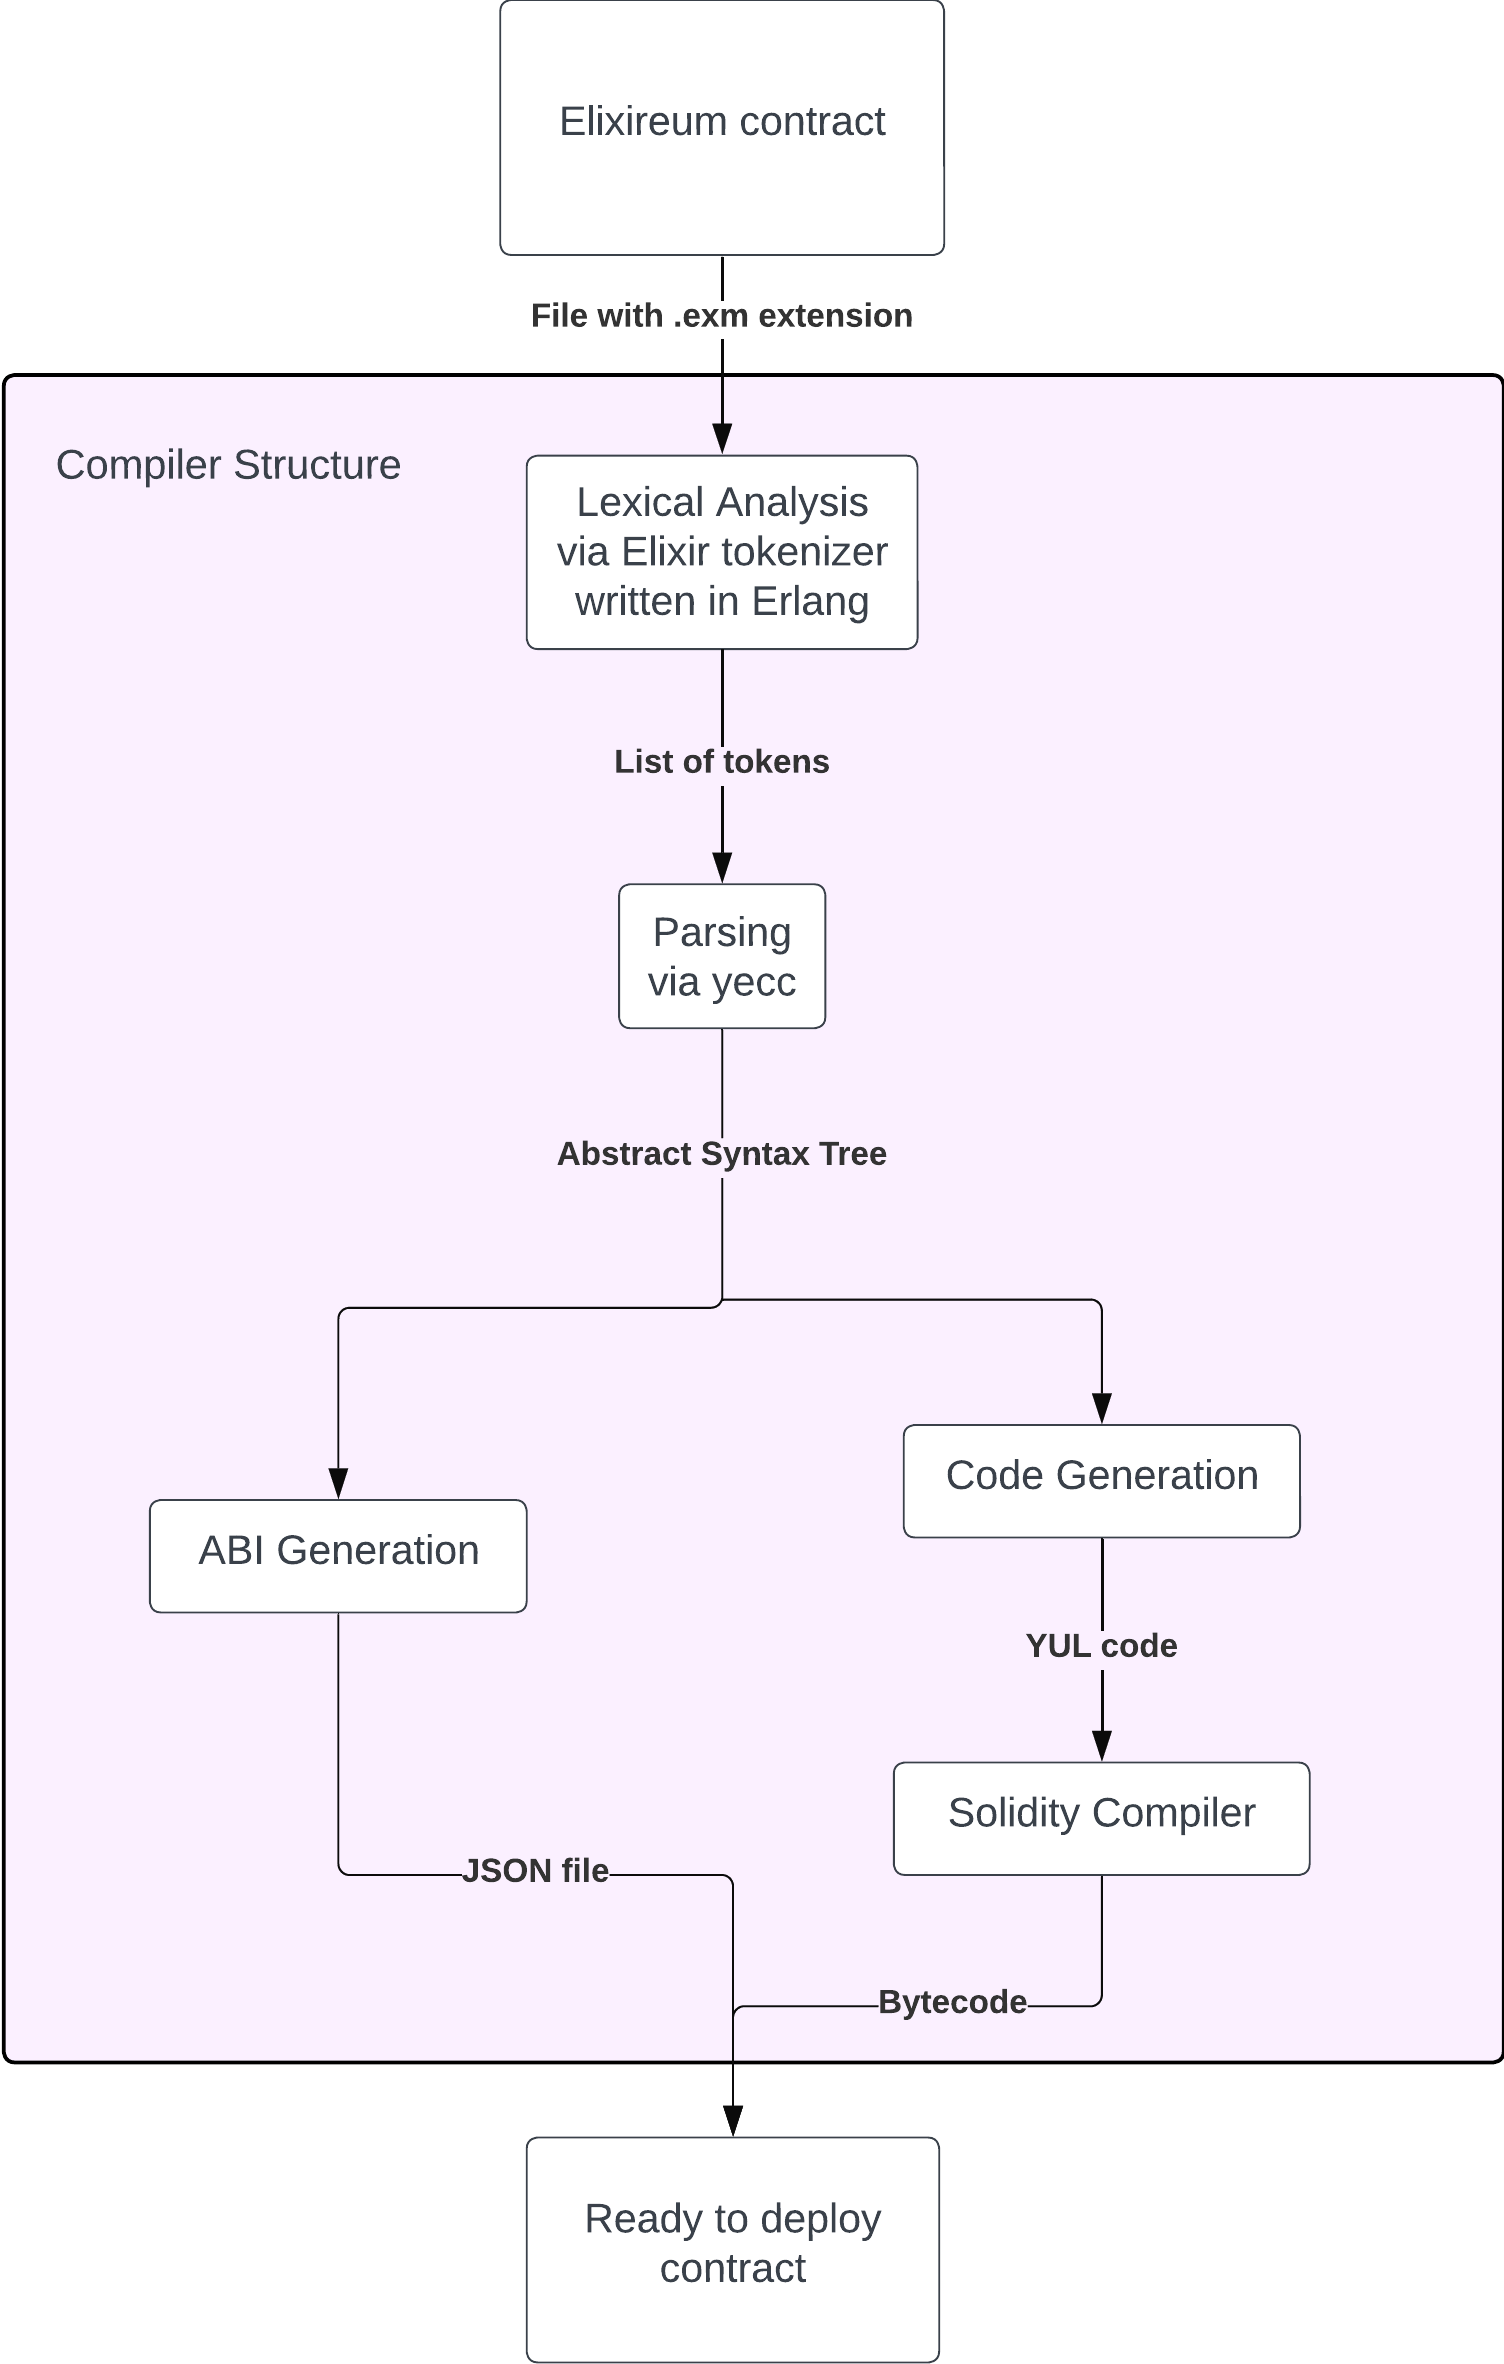
\includegraphics[width=0.8\textwidth]{figs/arch.png}
  \caption{Elixireum compiler architecture}
  \label{fig:arch}
\end{figure}

Here is the pipeline of actions performed by the main Compiler module, which can be seen visually in Fig. \ref{fig:arch}, each pipeline step is performed only if all the previous steps are successful.

\begin{itemize}
    \item Reading the source code from the file system.
    \item Running the Elixir tokenizer and parser on the source code.
    \item Performing the first pass of the Elixir AST in pre-order to gather information about defined functions, storage variables, and events, and packing this data into the following structure:
    
    \begin{lstlisting}[caption={Contract structure}, language=elixir, label={lst:contract_structure}]
      @type t :: %Contract{
          functions: Functions.t(),
          name: String.t(),
          private_functions: Functions.t(),
          variables: %{atom() => Variable.t()},
          events: %{atom() => Event.t()},
          aliases: %{atom() => list()}
        }
    \end{lstlisting}
    
    At this step, the compiler checks that public defined functions have corresponding typespecs\footnote{Typespec is the type specification of the function used in Elixir}, storage variables have types and events have all required fields.

    \item Perform the second traversal of the Elixir AST in post-order to generate Yul code.
    
    Specifically, this step generates a special function called a constructor. This function is executed at the deployment stage, and it takes its arguments not from calldata, but from the code. The Yul code that decodes arguments is generated using the calldata decoding module.

    Then, the compiler generates a function selector. The function selector is used to identify which function is being called based on the first four bytes of the call data. The first four bytes of the call data should be equal to the first four bytes of the Keccak256 hash of the string in the following format:
    \lstinline|function_name(1st_arg_type_name,2nd_arg_type_name,...)|
    constructed for the calling function, this is called method ID. For example, if the function has the following signature 
    \lstinline|transfer(address to, uint256 value)|
    Keccak256 is performed on 
    \lstinline|transfer(address,uint256)| The result of Keccak 256 is equal to 0xa9059cbb2ab0\dots So, the method ID for the transfer function is 0xa9059cbb. The function selector is simply a switch case expression where each public defined function corresponds to a case with its method ID. For each case statement, the compiler generates Yul code, responsible for function arguments decoding from call data, using the call data decoding module. Then the function call is generated as if it was a private function. Then, the compiler generates the code that encodes the value returned by the function into the return format using the return data encoding module.

    Then, the compiler generates Yul code for all user-defined functions, both public and private, since the difference between public and private functions is factored out into the function selector.

    Then, the compiler generates Yul code for standard functions used in user-defined functions. Standard functions are represented by the following structure:

    \begin{lstlisting}[caption={Standard function structure}, language=elixir, label={lst:standard_function_structure}]
      @type t :: %StdFunction{
          deps: %{atom() => t()},
          yul: String.t()
        }
    \end{lstlisting}

    The field deps represents other standard functions used by this standard function. This mechanism allows the definition of standard functions on demand, thus reducing the size of the Yul code and lowering the cost of deployment. Here is the mechanism that resolves dependencies:


    \begin{lstlisting}[caption={Standard function dependencies}, language=elixir, label={lst:standard_function_dependencies}]
    defp generate_std_functions(used_std_functions, definitions \\ %{}) do
      used_std_functions |>
      Enum.reduce(definitions, fn {function_name,
                                  %StdFunction{yul: yul, deps: deps}},
                                  definitions_acc ->
        {_, not_defined_deps} = Map.split(deps, Map.keys(definitions_acc))

        generate_std_functions(not_defined_deps, Map.put_new(definitions_acc, function_name, yul))
      end)
    end
    \end{lstlisting}
      
    
    \item Then, using the output of the first pass, the compiler generates ABI via ABI generator module.

\end{itemize}

\subsection{ABI generator}
\label{ssec:abi_generator}
The ABI generator takes the contract information collected by the compiler in the form of the contract structure \ref{lst:contract_structure} and generates a JSON ABI using the functions and events fields of the contract structure.


\subsection{Calldata decoding}
\label{ssec:calldata_decoding}
The call data decoding module recursively generates code for parsing arguments using information from the typespec of the function. The main function of this module is the decode function. It is generalized in terms of functions that perform loading and copying of data in order to reuse this function not only for argument decoding in calls, but also for argument decoding in the constructor where arguments are stored in memory, not in calldata. Here is an example of the base case of the decode function:

\begin{lstlisting}[caption={Calldata decoding base case}, language=elixir, label={lst:calldata_decoding_base}]
  def decode(
    _arg_name,
    %Type{encoded_type: encoded_type} = type,
    data_load_fn,
    _data_copy_fn,
    calldata_var,
    _init_calldata_var
  )
  when encoded_type > 69 and encoded_type < 102 do
    """
    mstore8(memory_offset$, #{type.encoded_type})
    memory_offset$ := add(memory_offset$, 1)
    mstore(memory_offset$, #{data_load_fn}(#{calldata_var}))
    memory_offset$ := add(memory_offset$, #{type.size})
    #{calldata_var} := add(#{calldata_var}, 32)
    """
  end
\end{lstlisting}

This function clause generates code that copies the value from calldata to memory and store the type for the Bytes<N> ABI type.

Here is an example of the recursive case of the decode function:

\begin{lstlisting}[caption={Calldata decoding recursive case}, language=elixir, label={lst:calldata_decoding_recursive}]
  def decode(
        arg_name,
        %Type{
          encoded_type: 3,
          components: components,
          size: size
        } = type,
        data_load_fn,
        data_copy_fn,
        calldata_var,
        init_calldata_var
      ) do
    tail_offset_var_name = "#{calldata_var}$#{arg_name}"
    init_tail_offset_var_name = "#{init_calldata_var}$#{arg_name}_init"

    """
    mstore8(memory_offset$, #{type.encoded_type})
    memory_offset$ := add(memory_offset$, 1)
    mstore(memory_offset$, #{Enum.count(components)})
    memory_offset$ := add(memory_offset$, 32)

    #{if size == :dynamic do
      """
      let #{tail_offset_var_name} := add(#{init_calldata_var}, #{data_load_fn}(#{calldata_var}))
      """
    else
      """
      let #{tail_offset_var_name} := #{calldata_var}
      """
    end}

    let #{init_tail_offset_var_name} := #{tail_offset_var_name}

    #{for {component, index} <- Enum.with_index(components) do
      decode(arg_name <> "#{index}", component, data_load_fn, data_copy_fn, tail_offset_var_name, init_tail_offset_var_name)
    end}
    """
  end
\end{lstlisting}

This function clause recursively generates code that copies the value from calldata to memory and stores type for the tuple ABI type. However, it only considers the tuple structure, i.e., the number of elements in it, and not the types of the elements, each element is decoded recursively.
  
\subsection{Emitting event}

The Event module is responsible for preparing and emitting events. Function emit, which is the main function of the module, takes the event as argument in the following form:

\begin{lstlisting}[language=elixir, caption={Event structure}, label={lst:event_structure}]
  @type t :: %Event{
          name: atom(),
          indexed_arguments: [keyword(Type.t())],
          data_arguments: [keyword(Type.t())],
          keccak256: String.t()
        }
\end{lstlisting}
  
An event has its signature, similar to a method ID for functions, but an event signature is the full Keccak256 hash of the following format:
$$event\_name(1st\_arg\_type\_name,2nd\_arg\_type\_name,...)$$

Events have indexed and data arguments. Indexed arguments are placed in the topics of the log. Topics are used to filter logs when fetching them from the blockchain. However, a log can have only up to four topics, with the first one being the event signature, so an event can have up to three indexed arguments. The size of the topics is limited to 32 bytes. For values larger than 32 bytes, its Keccak256 hash is used. The other data could be stored as data arguments that are placed in the data field of the log, with any value stored as is. The module generates code for encoding Elixireum values into indexed and data arguments. The function encode\_indexed\_argument is responsible for encoding indexed arguments. Here is the clause for types that are smaller than 32 bytes and are placed in topics as is:

\begin{lstlisting}[language=elixir, caption={Encode word-size indexed argument}, label={lst:encode_indexed_argument}]
  defp encode_indexed_argument(
    arg_name,
    %Type{encoded_type: encoded_type} = type,
    %YulNode{yul_snippet_usage: yul_snippet_usage},
    compiler_state
  )
  when encoded_type not in [1, 3, 102, 103] do
    var_name = "indexed_#{arg_name}_keccak_var$"
    arg_name_pointer = "indexed_#{arg_name}_pointer$"

    {"""
    let #{arg_name_pointer} := #{yul_snippet_usage}

    #{Utils.generate_type_check(arg_name_pointer, encoded_type, "Wrong type for indexed argument #{arg_name}", compiler_state.uniqueness_provider)}

    #{arg_name_pointer} := add(#{arg_name_pointer}, 1)
    let #{var_name} := shr(#{8 * (32 - type.size)}, mload(#{arg_name_pointer}))
    """, var_name}  
  end
\end{lstlisting}

Here is the clause for types that do not fit in one word:

\begin{lstlisting}[language=elixir, caption={Encode compex type indexed argument}, label={lst:encode_indexed_argument}]
  defp encode_indexed_argument(
         arg_name,
         %Type{} = type,
         %YulNode{yul_snippet_usage: yul_snippet_usage},
         _compiler_state
       ) do
    init_var_name = "indexed_#{arg_name}_keccak_init$"
    var_name = "indexed_#{arg_name}_keccak_var$"
    arg_name_pointer = "indexed_#{arg_name}_pointer$"

    {"""
     let #{init_var_name} := offset$
     let #{arg_name_pointer} := #{yul_snippet_usage}
     #{do_encode_indexed_argument(type, arg_name_pointer, init_var_name, 0)}
     let #{var_name} := keccak256(#{init_var_name}, sub(offset$, #{init_var_name}))
     """, var_name}
  end
\end{lstlisting}

The function do\_encode\_indexed\_argument is used to convert and copy Elixireum values to the format for Keccak256 and subsequent use in topics. It is defined recursively, similar to the calldata decode function.


The function encode\_data\_argument generates code that encodes data arguments, it uses the Return data encoding module \ref{ssec:return_data_encoding}. 

\begin{lstlisting}[language=elixir, caption={Encode data argument}, label={lst:encode_data_argument}]
  defp encode_data_argument(
         arg_name,
         %Type{} = type,
         %YulNode{yul_snippet_usage: yul_snippet_usage},
         index
       ) do
    """
    let #{arg_name}_$ := processed_return_value$
    let #{arg_name}_init$ := #{arg_name}_$
    let #{arg_name}_where_to_store_head$ := add(processed_return_value_init$, #{index * 32})
    return_value$ := #{yul_snippet_usage}
    #{Return.encode(type, "i$", "size$", "#{arg_name}_where_to_store_head$", "where_to_store_head_init$")}
    """
  end
\end{lstlisting}


\subsection{Return data encoding}
\label{ssec:return_data_encoding}

The Return data encoding module is responsible for encoding the value returned by an Elixireum function to an ABI format according to the typespec. It uses a similar approach to the calldata decoding module, but in the opposite way. The main function of this module is encode. Here is the base case of this function for simple types:

\begin{lstlisting}[language=elixir, caption={Encode base case}, label={lst:encode_base_case}]
  def encode(
    %Type{encoded_type: encoded_type, size: byte_size},
    _i_var_name,
    _size_var_name,
    where_to_store_head_var_name,
    _where_to_store_head_init_var_name
  )
  when encoded_type > 69 and encoded_type < 102 do
    offset = 8 * (32 - byte_size)

    """
    #{Utils.generate_type_check(...)}

    return_value$ := add(return_value$, 1)

    mstore(#{where_to_store_head_var_name}, shl(#{offset}, shr(#{offset}, mload(return_value$))))
    #{where_to_store_head_var_name} := add(#{where_to_store_head_var_name}, 32)

    return_value$ := add(return_value$, #{byte_size})
    """
  end
\end{lstlisting}

Here is an example of a recursive case:

\begin{lstlisting}[language=elixir, caption={Encode recursive case}, label={lst:encode_recursive_case}]
  def encode(
        %Type{
          encoded_type: 103 = encoded_type,
          items_count: size,
          components: [components]
        },
        i_var_name,
        size_var_name,
        where_to_store_head_var_name,
        where_to_store_head_init_var_name
      )
      when is_integer(size) do
    """
    #{Utils.generate_type_check(...)}

    return_value$ := add(return_value$, 1)
    let #{size_var_name} := mload(return_value$)

    #{Utils.generate_value_check(...)}

    return_value$ := add(return_value$, 32)

    for { let #{i_var_name} := 0 } lt(#{i_var_name}, #{size_var_name}) { #{i_var_name} := add(#{i_var_name}, 1) } {
      #{encode(components, i_var_name <> "_", size_var_name <> "_", where_to_store_head_var_name, where_to_store_head_init_var_name)}
    }
    """
  end
\end{lstlisting}
    